\documentclass[lettersize,journal]{IEEEtran}
\usepackage{amsmath,amsfonts}
\usepackage{amssymb}
\usepackage{algorithmic}
\usepackage{algorithm}
\usepackage{array}
%\usepackage[caption=false,font=normalsize,labelfont=sf,textfont=sf]{subfig}
\usepackage{textcomp}
\usepackage{stfloats}
\usepackage{url}
\usepackage{verbatim}
%\usepackage{graphicx}
\usepackage{tikz}
\usepackage[font=footnotesize]{caption}
\usepackage[font=footnotesize]{subcaption}
\usepackage{cite}
% updated with editorial comments 8/9/2021

%% package for urls
\usepackage{url}

%% hyperref
% and an override to make hyperref work with ieeeconf.cls
\makeatletter
\let\NAT@parse\undefined
\makeatother
\usepackage[pagebackref=true,breaklinks=true,colorlinks,bookmarks=false]{hyperref}
\makeatletter
\newcommand*{\textlabel}[2]{%
  \edef\@currentlabel{#1}% Set target label
  \phantomsection% Correct hyper reference link
  #1\label{#2}% Print and store label
}
\makeatother

\usepackage{textpos}
\usepackage{amsthm}

%% correct bad hyphenation here
\hyphenation{obs-tacles}

\renewcommand{\qedsymbol}{$\blacksquare$}

\theoremstyle{definition}
\newtheorem{thm}{Theorem}[section]
\newtheorem{lem}[thm]{Lemma}
\newtheorem{prop}[thm]{Proposition}
\newtheorem{assm}[thm]{Assumption}
\newtheorem{cor}{Corollary}
\newtheorem{conj}{Conjecture}[section]
\newtheorem{defn}{Definition}[section]
\newtheorem{exmp}{Example}[section]
\newtheorem*{pb}{Problem}%[section]
\newtheorem{rem}{Remark}
\newtheorem{obs}{Observation}
\newtheorem*{ctb}{Contribution}

\DeclareMathOperator*{\argmax}{arg\,max}
\DeclareMathOperator*{\argmin}{arg\,min}


\begin{document}
\bstctlcite{IEEEexample:BSTcontrol}

\title{A Low-Cost Approach for Real-Time Autonomous Large-Scale Exploration}%, 3D~Reconstruction, and Mapping}

\author{Adam Seewald${}^\text{1}$, Marvin Chanc{\'a}n${}^\text{1}$, Connor M. McCann${}^\text{2}$, Seonghoon Noh${}^\text{1}$, Omeed Fallahi${}^\text{1}$, Hector Castillo${}^\text{1}$, Ian Abraham${}^\text{1}$, and Aaron M. Dollar${}^\text{1}$%~\IEEEmembership{Staff,~IEEE,}
        % <-this % stops a space
  \thanks{Manuscript received: Month, Day, Year; Revised Month, Day, Year; Accepted Month, Day, Year.}%Use only for final RAL version
  \thanks{This paper was recommended for publication by Editor Editor A. Name upon evaluation of the Associate Editor and Reviewers' comments.} %Use only for final RAL version
  \thanks{${}^\text{1}$A.\hspace*{.4ex}S., C.\hspace*{.4ex}M., S.\hspace*{.4ex}N., O.\hspace*{.4ex}F., H.\hspace*{.4ex}C, I.\hspace*{.4ex}A., and A.\hspace*{.4ex}M.\hspace*{.4ex}D. are with the Department of Mechanical Engineering and Materials Science, Yale University, CT, USA. Email: {\tt\footnotesize \href{mailto:adam.seewald@yale.edu}{adam.seewald@yale.edu};}}
  \thanks{${}^\text{2}$C.\hspace*{.4ex}M.\hspace*{.4ex}C. is with the School of Engineering and Applied Sciences, Harvard University, MA, USA.}
  \thanks{Digital Object Identifier (DOI): see top of this page.}
}

% The paper headers
\markboth{Journal of \LaTeX\ Class Files,~Vol.~14, No.~8, August~2021}%
{Shell \MakeLowercase{\textit{et al.}}: A Sample Article Using IEEEtran.cls for IEEE Journals}

\IEEEpubid{0000--0000/00\$00.00~\copyright~2021 IEEE}
% Remember, if you use this you must call \IEEEpubidadjcol in the second
% column for its text to clear the IEEEpubid mark.

\maketitle
\vspace*{-1cm}
\begin{abstract} 
This letter describes an approach for autonomous large-scale exploration for robots with a lower sensory footprint. Requiring just an RGB-D camera and low-power computing hardware, the approach consists of a framework based on the open-source robot operating system middleware and an experimental robotic platform with rocker-bogie suspension. It operates in real-time, in unknown and GPS-denied environments, and indoor and outdoor challenging terrains. 
The exploration path is derived with a novel methodology that extends frontier- and sampling-based exploration literature with a path-following vector field and the position exploiting a state-of-the-art simultaneous localization and mapping algorithm. 
The framework allows the robot to explore its surroundings at lower frequencies and in real-time, utilizing cheaper hardware compared to state-of-the-art approaches, and is generic in terms of portability to other mobile robots with both computational and cost constraints. 
The framework further consists of a novel methodology to interact with a remotely located human operator based on an inexpensive long-range and low-power communication technology from the internet-of-things domain and a customized communication protocol. 
Data show improved performance per cost over the baseline of existing autonomous exploration %system-of-systems
approaches with indoor and outdoor experiments.
\end{abstract}

\begin{IEEEkeywords}
Article submission, IEEE, IEEEtran, journal, \LaTeX, paper, template, typesetting.
\end{IEEEkeywords}

%\section{Introduction}
%\IEEEPARstart{T}{his} file is intended to serve as a ``sample article file''
%for IEEE journal papers produced under \LaTeX\ using
%IEEEtran.cls version 1.8b and later. The most common elements are covered in the simplified and updated instructions in ``New\_IEEEtran\_how-to.pdf''. For less common elements you can refer back to the original ``IEEEtran\_HOWTO.pdf''. It is assumed that the reader has a basic working knowledge of \LaTeX. Those who are new to \LaTeX \ are encouraged to read Tobias Oetiker's ``The Not So Short Introduction to \LaTeX ,'' available at: \url{http://tug.ctan.org/info/lshort/english/lshort.pdf} which provides an overview of working with \LaTeX.

\section{Introduction}

\begin{figure}

\vspace*{-.5cm}
  \input{figures/_rb5_abstract.pdf_tex}
  \caption{A robot needs to explore its surroundings with a lower sensory and computing footprint compared to state-of-the-art approaches--the picture illustrates an experimental robotic platform that carries an RGB-D camera and a low-power computing unit to derive an exploratory coverage path on a large-scale, in real-time, and in both indoor and outdoor challenging terrains.}
  \vspace*{-.6cm}
  \label{fig:0}
\end{figure}

\IEEEPARstart{W}{idely} used in cluttered environments~\cite{kohlbrecher2014hector,kulkarni2022autonomous,tranzatto2022cerberus,kim2022autonomous}, mobile robots can both substitute~\cite{rubio2019review} and outperform humans in, e.g., areas that are too far or too dangerous to navigate~\cite{takahiro2022legged,roucek2020darpa,tabib2022autonomous,ebadi2020lamp}. In these areas, robots are often required to identify their surroundings by sensing the environment~\cite{mei2006energy} and planning and executing complex trajectories~\cite{shrestha2019learned,eldemiry2022autonomous}. With little or no human intervention~\cite{alatise2020review}, this problem is known in the literature as autonomous exploration~\cite{shrestha2019learned}. 
While successful in challenging indoor and outdoor environments~\cite{lluvia2021active,placed2022survey}, 
autonomous exploration is especially useful in dynamic environments with no prior knowledge of the space to be covered~\cite{bircher2016receding,rubio2019review}.
Despite recent advancements, autonomy is limited and costly in such environments. 
Many approaches that tackle autonomous exploration 
integrate commercial robots with sensing equipment that is both prohibitively expensive and difficult to maintain~\cite{lluvia2021active,placed2022survey,muller2021openbot,tabib2022autonomous,tardioli2019ground,ebadi2020lamp,dang2019graph,surmann2003autonomous}. 
\IEEEpubidadjcol
There is a wide range of methodologies for autonomous exploration at present~\cite{placed2022survey,julia2012comparison} nonetheless, which span from algorithmic foundations~\cite{yamauchi1997frontier,placed2022survey,dang2019graph} to system-of-systems frameworks where, e.g., a multitude of robots integrate existing algorithms with sensors for real-time large-scale exploration~\cite{tranzatto2022cerberus,roucek2020darpa,tardioli2019ground,tabib2022autonomous,ebadi2020lamp}. 
Recent efforts in this direction include low-cost robots for exploration~\cite{muller2021openbot, zhou2021smartphone,faisal2021low} but lack terrain adaptability~\cite{muller2021openbot} and %computational 
capabilities~\cite{zhou2021smartphone,faisal2021low} often required to navigate outdoors in the real-world~\cite{rubio2019review,kulkarni2022autonomous}.

Furthermore, in areas that are ambiguous or challenging to traverse--albeit autonomous--state-of-the-art approaches rely on humans for supervision and high-level decision-making~\cite{tranzatto2022cerberus,roucek2020darpa,tabib2022autonomous}. 
As a result, robots often operate close to humans or require expensive network equipment, such as a mesh of communication devices~\cite{tranzatto2022cerberus,kulkarni2022autonomous,ebadi2020lamp}, or existing network infrastructure~\cite{khairuldanial2019mobile,baek2022ros,voigtlander20175g}, thereby restricting autonomous exploration to indoor settings only~\cite{delgado2022oros,cadena2016past,eldemiry2022autonomous,corah2019communication,papachristos2017uncertainty}.
Conversely, our methodology exploits LoRa--an inexpensive long-range and low-power communication technology~\cite{shanmuga2020survey} from the internet-of-things domain--with a customized communication protocol 
for human intervention in, e.g., the eventuality of the robot being unable to move with the local sensory information. 

Starting from the cost advantages of LoRa communication, we develop here a low-cost approach consisting of an exploration framework based on the open-source robot operating system (ROS) middleware~\cite{quigley2009ros} and an experimental robotic platform--RB5 in Figure~\ref{fig:0}, a mobile robot with rocker-bogie suspension--capable of exploring autonomously dynamic indoor and outdoor environments.
Similar platforms in the literature comprise two degrees of freedom suspension with pivots~\cite{setterfield2013terrain,mann2005dynamic,faisal2021low} and provide rough terrain static adaptability~\cite{kim2012optimal}. They are cheaper than, e.g., legged robots in terms of cost per unit and operation, as they are able to overcome obstacles without costly computations for gait adaptation and planning~\cite{muller2021openbot}.
Although specific to RB5 in the letter, the approach is generic in terms of portability to other mobile robots with cost and computational constraints.
%
Hardware-wise, the approach maintains a lower sensory footprint with low-cost components, whereas 
software-wise, it integrates multiple modules into the exploration framework. Being able to operate in both unknown and GPS-denied environments, the approach derives the robot's position using a state-of-the-art simultaneous localization and mapping (SLAM) algorithm~\cite{labbe2019rtab} %,campos2021orb}, 
and the trajectory with a novel methodology that extends exploration literature with a path-following vector field~\cite{goncalves2010vector} from the aerial robotics domain~\cite{seewald2022energy,garcia2017guidance,seewaldphdthesis}. This allows the robot to explore its surroundings at lower frequencies and in real-time, utilizing cheaper computing hardware compared to state-of-the-art approaches~\cite{placed2022survey,tabib2022autonomous,ebadi2020lamp,dang2019graph}. 

The remainder of the letter is structured as follows. In Section~\ref{sec:fe}, data show %improved ``coverage per cost'' 
the exploration performance and obstacle avoidance features 
over the baseline of existing autonomous exploration system-of-systems with indoor and outdoor ``in the field'' experiments. 
Sec.~\ref{sec:m} describes the approach from the software and hardware standpoints. Sec.~\ref{sec:rw} summarizes and compares existing literature, Sec.~\ref{sec:pf} formalizes the problem of autonomous exploration, and Sec.~\ref{sec:cf} drafts conclusions %a proposes 
and future directions.

%Utilizing the advantages of LoRa for long-range communication, we propose the mechanical design and the  
%%%%%

\section{Related Work}
\label{sec:rw}

Literature that tackles autonomous exploration is broad and diverse~\cite{lluvia2021active,placed2022survey,julia2012comparison}, yet, most approaches use expensive sensing equipment such as LiDARs~\cite{kohlbrecher2014hector,kulkarni2022autonomous,tranzatto2022cerberus,roucek2020darpa,ebadi2020lamp,tardioli2019ground,dang2019graph,batinovic2021multi} and laser range finders~\cite{kim2022autonomous,surmann2003autonomous}. 
Even though approaches that utilize cheaper sensors, such as RGB depth (RGB-D) cameras~\cite{tranzatto2022cerberus,kim2022autonomous,roucek2020darpa,tabib2022autonomous,ebadi2020lamp,eldemiry2022autonomous,bircher2016receding,papachristos2017uncertainty,dai2020fast}, RGB cameras~\cite{zhou2021smartphone,dang2019graph,muller2021openbot}, and sonars~\cite{zhou2021smartphone,muller2021openbot}, are studied, they often operate along other more expensive equipment~\cite{dang2019graph,ebadi2020lamp,roucek2020darpa,kim2022autonomous,tranzatto2022cerberus} or indoors only~\cite{bircher2016receding,eldemiry2022autonomous,dai2020fast,papachristos2017uncertainty,zhou2021smartphone}, and have limited autonomy~\cite{bircher2016receding,papachristos2017uncertainty,dai2020fast} or obstacle avoidance features~\cite{zhou2021smartphone,muller2021openbot}.
Recent approaches minimize exploration costs nonetheless~\cite{muller2021openbot,zhou2021smartphone,tabib2022autonomous,eldemiry2022autonomous,bircher2016receding} by, e.g., exploiting sensing capabilities of commercial smartphones~\cite{muller2021openbot,zhou2021smartphone} or using case-specific aspects~\cite{tabib2022autonomous} but are generally unable to operate in a wide variety of challenging %indoor and outdoor
environments.
%
It is such a state of practice that has prompted us to propose a low-cost approach to autonomous exploration. Similar to recent literature, it can operate on a large scale but with a lower sensory footprint--an RGB-D camera to sense the environment--and in a variety of terrains both indoors and outdoors.

Software-wise, recent efforts into autonomous exploration often require expensive prior learning~\cite{shrestha2019learned} or run on multiple agents~\cite{kulkarni2022autonomous,tranzatto2022cerberus,roucek2020darpa}, whereas %general 
approaches with little computing resources are scarce~\cite{bircher2016receding,batinovic2021multi,faisal2021low,muller2021openbot}. More traditional approaches such as these based on frontiers~\cite{kim2022autonomous,roucek2020darpa,batinovic2021multi}, graphs~\cite{kulkarni2022autonomous,tranzatto2022cerberus,dang2019graph}, grids~\cite{corah2019communication,tabib2022autonomous}, and random trees~\cite{papachristos2017uncertainty} are also studied, but mixed approaches are to be preferred~\cite{kohlbrecher2014hector,mei2006energy,shrestha2019learned,bircher2016receding,surmann2003autonomous,wenchuan2019sampling} to maximize performance and resources~\cite{placed2022survey,bircher2016receding}.
%
Similarly, we propose a mixed approach. A frontier-based method that exploits the scarcity of resources while still running in real-time with comparable autonomy and obstacle avoidance features to its more expensive counterparts~\cite{roucek2020darpa,tranzatto2022cerberus,kim2022autonomous,dang2019graph}.

%These approaches solve the exploration with different techniques, which are generally grouped by the exploration planning methodology. Some recent approaches study learning~\cite{}


\section{Problem Formulation}
\label{sec:pf}

The problem considered in this work to showcase the approach for large-scale exploration is that of exploring a bounded volume $\mathcal{Q}\subseteq\mathbb{R}^3$ with respect to an inertial navigation frame $\mathcal{O}_W$. If the notation $[n]$ denotes a set with positive naturals up to $n$ and $[n]_{>0}$ with strictly positive naturals, we are interested in collision-free trajectories that explore $\mathcal{Q}$ and avoid $i\in[n]_{>0},n\in\mathbb{N}_{\geq 0}$ obstacles $\mathcal{Q}^{O_i}\subset\mathbb{R}^3$. We can approximate the space that delimits $\mathcal{Q}$ and $\mathcal{Q}^{O_i}$ for each $i$ with a set of vertices within which the two sets are contained.

\begin{pb}[Exploration]
  Consider sets of vertices $V:=\{\mathbf{v}_1,$ $\mathbf{v}_2,\dots\}$, $O_i:=\{\mathbf{o}_{i,1},\mathbf{o}_{i,2},\dots\}$ with $i\in[n],\mathbf{v}_j,\mathbf{o}_{i,k}\in\mathbb{R}^2,$ $\forall j\in[|v|],\,k\in[|o_i|]$ a point w.r.t. $\mathcal{O}_W$. Let $V$ enclose $\mathcal{Q}$, $O_i$ $\mathcal{Q}^{O_i}$ per each $i$. The \textit{exploration problem} is the problem of finding the coverage that visits each point $\mathbf{p}\in\mathcal{Q}\cap\mathcal{Q}^{O_1}\cap\mathcal{Q}^{O_2}\cap\cdots\cap\mathcal{Q}^{O_n}:=\mathcal{Q}^V$.
\end{pb}

Here the notation $|\cdot|$ denotes the cardinality and $\mathbb{R}$, $\mathbb{Z}$ are reals and integers. Bold notation is used for vectors.

Let $\phi$ be a path function, i.e., a function the robot tracks as it explores its surroundings in $\mathcal{Q}^V$, avoiding the obstacles $\mathcal{Q}^{O_i}$.

\begin{defn}[Path function]\label{def:pf}
  $\phi:\mathbb{R}^2\rightarrow\mathbb{R}$ is a two-dimensional continuous and differentiable \textit{path function} of the $x$, $y$ components of $\mathbf{p}$.
\end{defn}

\begin{defn}[Coverage]\label{def:co}
  Given a tuple with a path function and its time component, $\langle\phi,t\rangle$, the \textit{coverage} is the collection of multiple tuples.
\end{defn}

The large-scale exploration framework (see Sec.~\ref{sec:le}) derives $\phi$ at each sampling step and adds it to the global ``coverage stack''. The process ends once $\mathcal{Q}^V$ is covered.

\section{Approach}
\label{sec:m}

The approach section details the implementation and design choices in terms of %both 
the software for autonomous large-scale exploration and the low-cost hardware in respectively Sec.~\ref{sec:le}~and~\ref{sec:md}.

\subsection{Autonomous large-scale exploration}
\label{sec:le}

\begin{figure*}
  \begin{subfigure}[m]{0.33\textwidth}
    \centering
    \input{figures/_GOPR0984.pdf_tex}
    \caption{Initial detection of an obstacle ``wheel'' with $\phi_{t_0}$ selected so that it avoids the obstacle.}
    \label{fig:3-1}
  \end{subfigure}
  \hfill
  \begin{subfigure}[m]{0.32\textwidth}
    \centering
    \hspace*{-.15cm}
    \input{figures/_GOPR0985.pdf_tex}
    \caption{The robot continues to track $\phi_{t_0}$ up to the next iteration. Here it finds a new trajectory $\phi_{t_1}$.}
    \label{fig:3-2}
  \end{subfigure}
  \begin{subfigure}[m]{0.33\textwidth}
    \centering
    \hspace*{.05cm}
    \input{figures/_GOPR0990.pdf_tex}
    \caption{The process continues up to when the entire space is explored.}
    \label{fig:3-3}
  \end{subfigure}
  \caption{The autonomous large-scale exploration framework consists of the robot sampling the environment and searching for obstacles and unexplored areas. The framework clusters the two groups into vertices sets and builds candidate path functions. From these, it selects the optimal trajectory w.r.t. a given cost and iterates the operation at each step. In between the iterations, it tracks the trajectory, saving computational and sensing resources.}
  \label{fig:3}
\end{figure*}

There is a large body of work for robot exploration~\cite{lavalle2006planning,yamauchi1997frontier,placed2022survey,dang2019graph,julia2012comparison}. 
While the majority exploits the concept of frontiers~\cite{wenchuan2019sampling}, i.e., boundaries between known and unknown space, mixed approaches are emerging~\cite{dai2020fast,schmid2020efficient,placed2022survey}. 
Especially useful in the presence of diverse sensing modalities, e.g., involving raw sensory data, topologies, semantics, etc., they have multiple %potential 
advantages for real-world environments~\cite{placed2022survey,batinovic2021multi}. 
%
We propose a %one 
mixed approach for our large-scale exploration framework, combining frontier- and sampling-based methods, similar to some recent approaches~\cite{dai2020fast,wenchuan2019sampling},~\cite{dang2019graph}. % forcing latex not to split lines...

The framework evaluates local frontiers at each step, samples the environment, and determines feasible candidate path functions $\phi$ that intersect $\mathcal{Q}^V$ (see Definition~\ref{def:pf}).
The next $\phi$ is selected so that the frontier is the largest, but other costs are possible (see Sec.~\ref{sec:cf}). 
The framework then derives a path-following vector field that points to $\phi$ at any point and guides the robot utilizing the gradient descent algorithm. This allows the robot to, e.g., follow the covering path for longer and in real-time compared to approaches that utilize frontiers only, decreasing computational and cost requirements (see Sec.~\ref{sec:fe}).

To derive the path-following vector field, let the gradient of $\phi$ be defined
\begin{equation}\small
  \nabla\phi:=\begin{bmatrix}
    \partial\phi(\mathbf{p})/\mathbf{p}_x\\
    \partial\phi(\mathbf{p})/\mathbf{p}_y
  \end{bmatrix},
\end{equation}
where $\partial\phi/\mathbf{p}$ is the differential, and $\mathbf{p}_x$, $\mathbf{p}_y$ are the $x$ and $y$ compoenents of $\mathbf{p}$.
It points in the direction where $\phi$ maxi-mally locally increases. To assign the direction to each point, we use the construct of vector fields, which is common in other motion planning literature~\cite{lavalle2006planning,garcia2017guidance,goncalves2010vector}
\begin{equation}\label{eq:vecf}
  \Phi(t,\phi):={\textstyle \bigcup\limits_{\mathbf{p}(t)\in\mathcal{Q}}}\nabla\phi(\mathbf{p}(t)).
\end{equation}

We modify the vector field in Equation~(\ref{eq:vecf}) to point to the contour of the path function $\phi$ rather than its local maxima
\begin{equation}\label{eq:pfvf}
  \Delta\phi(\mathbf{p}(t)):=E\nabla\phi(\mathbf{p}(t))-k_e\phi(\mathbf{p}(t))\nabla\phi(\mathbf{p}(t)),
\end{equation}
where $E\nabla\phi$ points perpendicularly to the gradient and $\phi\nabla\phi$ to $\phi$ at $k_e\in\mathbb{R}_{>0}$ rate~\cite{garcia2017guidance}. $E$ is the following direction, i.e.,
\begin{equation}\small
  E=\begin{bmatrix}
    1 & 0\\ 0 & -1
  \end{bmatrix},
\end{equation}
is counterclockwise and $-E$ clockwise directions~\cite{seewaldphdthesis}.

Let thus the path-following equivalent of Eq.~(\ref{eq:vecf}) be 
\begin{equation}
  \Phi_\phi(t,\phi):={\textstyle \bigcup\limits_{\mathbf{p}(t)\in\mathcal{Q}}}\Delta\phi(\mathbf{p}(t)).
\end{equation}


\begin{algorithm}[t]
  \begin{algorithmic}[1]
    \small
    \FORALL{$t\in\mathcal{T}$}
      \STATE \textbf{if} $\mathcal{P}\cap\mathcal{Q}=\{\varnothing\}$ \textbf{then return }$\langle\phi,t\rangle$\vspace*{.3ex}\label{alg:cs}
      \STATE $\mathcal{Q}^V_t:=O_{1,t},O_{2,t},\dots,O_{n,t},V_t\gets$ sensor readings\label{alg:vd}\vspace*{.3ex}
      \IF{$\mathcal{Q}_t^V\neq\mathcal{Q}_{t-1}^V$}\vspace*{.3ex}
        \STATE $\{\phi_{1,t},\phi_{2,t},\dots\}\gets$ $\phi$s in Def.~\ref{def:pf}, inters. $\mathcal{Q}^V\cap \Psi(\mathcal{Q}^V_t)$\label{alg:vp}\vspace*{.3ex}
        \STATE \textbf{if} $\phi_t:=\{\phi_{1,t},\phi_{2,t},\dots\}=\{\varnothing\}$ \textbf{then }the robot is stuck\label{alg:mpty}\vspace*{.3ex}
        \STATE \textbf{else}
        \STATE $\,\,\,\,\,\,\phi_t\gets \argmax_{\phi}l(\phi_t,t,\mathcal{Q}_t^V)$ in Eq.~(\ref{eq:cost})\label{alg:am}\vspace*{.3ex}
        \STATE $\,\,\,\,\,\,\langle\phi,t\rangle\gets\langle\phi,t\rangle\cup\langle\phi_t,t\rangle$ in Def.~\ref{def:co}\vspace*{.3ex}
        \STATE $\,\,\,\,\,\,\mathcal{P}\gets\mathcal{P}\cup \Psi(\mathcal{Q}_t^V)$
        \STATE \textbf{end if}
        \vspace*{.3ex}
      \ENDIF
      \STATE $\varphi(t,\mathbf{p}(t))\gets\varphi(t-1,\mathbf{p}(t-1))+\theta\Delta\phi(\mathbf{p}(t))$ in Eq.~(\ref{eq:pfvf})\vspace*{.3ex}\label{alg:vf}
    \ENDFOR
  \end{algorithmic}
  \caption{Derivation of the exploration coverage $\langle\phi,t\rangle$}\label{alg}
\end{algorithm}

The path-following vector field is summarized in the pseudo-code in Algorithm~\ref{alg}, with the gradient descent in Line~\ref{alg:vf}. The vector $\varphi\in\mathbb{R}^2$ points the robot in the direction of the path function $\phi$ with a scalar step size $\theta\in\mathbb{R}_{>0}$. The algorithm runs at the highest frequency $\mathcal{T}:=\{t_0,t_0+h,\dots\}$ with a time-step $h\in\mathbb{R}_{>0}$. Practically, there might be different $h$s at different times (see Sec.~\ref{sec:fe}). In Line~\ref{alg:cs}, the algorithm evaluates if the bounded volume $\mathcal{Q}$ is covered utilizing the covered volume $\mathcal{P}\subseteq\mathbb{R}^3$. The latter is updated in Line~\ref{alg:vp}, where the function $\Psi:\mathbb{R}^{2n}\times\mathbb{R}^2\rightarrow\mathbb{R}^{3n}\times\mathbb{R}^3$ maps the vertices to the volume. The vertices of $\mathcal{Q}^V_t$ in Line~\ref{alg:vd} are derived from sensor readings, assuming the presence of a low-cost depth camera. The framework read the camera's point cloud, clustering the obstacles $O_{1,t},O_{2,t},\dots$ by checking if the distance between consecutive points in space is within a given threshold $\varepsilon\in\mathbb{R}_{>0}$ and deriving their vertices. The vertices of the space at time instant $t$, $V_t$ are simply the limits of the sensor's field of view.

The remaining lines %in the algorithm
compute the feasible path functions $\{\phi_{1,t},\phi_{2,t},\dots\}$ by intersecting the space $\Psi(\mathcal{Q}^V_t)$ with possible candidate trajectories that have their final points laying at the edges of $\mathcal{Q}^V_t$, i.e., splines of the form
\begin{equation}\label{eq:spln}
  a(x-\mathbf{p}_x)^3+b(x-\mathbf{p}_x)^2+c(x-\mathbf{p}_x)+d-y=0,
\end{equation}
where $a,b,c\in\mathbb{R}$ are the coefficients of the spline. 
The best trajectory is then derived via the cost $l$ in Line~\ref{alg:am}, utilizing the intersection of the largest frontier. For instance, if there are no obstacles, Eq.~(\ref{eq:spln}--\ref{eq:cost}) are such that $\phi$ is a line parallel to the direction of the robot. Formally
\begin{equation}\label{eq:cost}\small
  l\hspace*{-.5ex}:=\hspace*{-.5ex}\bigl\{\lVert \mathbf{p}_1\hspace*{-.5ex}-\mathbf{p}_2\rVert\,|\,\exists\,\mathbf{p}_1,\hspace*{-.5ex}\mathbf{p}_2\hspace*{-.5ex}\in\hspace*{-.5ex}\Psi(\mathcal{Q}_t^V)\text{\hspace*{.5ex}s.t.\hspace*{.5ex}}\mathbf{p}_1\hspace*{-.5ex}\neq\hspace*{-.5ex}\mathbf{p}_2,\phi(\mathbf{p}_1-\mathbf{p}_2)\hspace*{-.5ex}\approx\hspace*{-.5ex}0\bigr\},
\end{equation}
where the condition $\phi(\mathbf{p}_1-\mathbf{p}_2)$ is evaluated on a given $\varepsilon\in\mathbb{R}_{>0}$, i.e., $|\phi(\mathbf{p}_1-\mathbf{p}_2)|<\varepsilon$.

Using the algorithm, the framework provides a way to explore space $\mathcal{Q}$ and avoid obstacles $\mathcal{Q}^{O_i}$. There are configurations at which there are no feasible trajectories nonetheless, e.g., if $\{\phi_{1,t},\phi_{2,t},\dots\}=\{\varnothing\}$ in Line~\ref{alg:mpty}. In this scenario, the framework allows a human to intervene via standard wireless and LoRa communication technology. The robot can then be teleoperated on long distances--studies from the internet-of-things domain~\cite{shanmuga2020survey,raza2017lora} report a range of up to five kilometers in an urban setting--and with a relatively inexpensive hardware equipment (two LoRa bundles). The framework we propose utilizes a web interface to parse human commands into our custom communication protocol which utilizes the LoRa physical layer's payload to transfer $\varphi$'s $x$ and $y$ components.

The algorithm is illustrated in Fig.~\ref{fig:3}. At each iteration, the robot samples the environment and derives a set of possible candidate trajectories $\{\phi_{1,t},\phi_{2,t},\dots\}$. If there is no obstacle ahead, the optimal trajectory per iteration $\phi_t$ is a line parallel to the robot's direction of travel (see Fig.~\ref{fig:3-3}). If there are obstacles, the framework selects the trajectory via the cost $l$, $\phi_t$, which goes through the middle of the largest frontier (see Fig.~\ref{fig:3-1}~and~\ref{fig:3-2} for respective obstacles ``wheel'' and ``wall'').

To derive a map of the environment and to keep the track of the robot within it in Line~\ref{alg:vf}, the framework uses a state-of-the-art visual SLAM algorithm from the literature~\cite{labbe2019rtab}. The robot's location is also used to determine whether the exploration is complete in Line~\ref{alg:cs}% and to asses exploration-to-cost (see Fig.~\ref{})
, showing that the algorithm is effective in exploring unknown environments with a lower sensory footprint (see Sec.~\ref{sec:fe}). Furthermore, earlier iteration of the work exploited a different SLAM algorithm from the visual SLAM community~\cite{campos2021orb}, showing that some of the framework components are interchangeable.

The framework %we propose 
is distributed under the popular open-source CC BY-NC-SA license\footnote{{\tt\footnotesize \href{https://github.com/adamseew/ytcg_ground-based}{github.com/adamseew/ytcg\_ground-based}}}. It is composed of three distinct components. A ``ground robot'' ROS2~\cite{quigley2009ros} package implements the communication with a base station using either the IEEE 802.11 wireless communication or long-range LoRa protocols. The package further implements the serial communication with the microcontroller implemented in Arduino and the vertices detection (see Algorithm~\ref{alg}). A ``ground navigation'' ROS package collects point clouds from an RGB-D sensor (an Intel (R) RealSense (TM) Depth Camera~\cite{keselman2017intel} D435) and other data from the SLAM algorithm~\cite{labbe2019rtab} and ports them into ROS2. Finally, a ``base server'' implements the necessary functionality for remote human intervention.
Both ``ground robot'' and ``ground navigation'' are implemented in C++ in ROS2 and ROS respectively, whereas ``base station'' is in PHP and JavaScript.

\subsection{Low-cost hardware design}
\label{sec:md}

The RB5 mobile robot adopts a rocker-bogie suspension system~\cite{bickler1989articulated} found on NASA's rovers including Sojourner and Curiosity. On either side of the robot, an upside-down V-shaped linkage called the rocker pivots about an axis on the robot frame. The rocker has a wheel at one end and a smaller V-shaped linkage on the other arm. The smaller linkage, called the bogie, can pivot about an axis on the rocker and has two wheels at its tips. The articulated nature of the rocker-bogie suspension allows the mobile robot to adapt to uneven terrains~\cite{kim2012optimal,mann2005dynamic,faisal2021low} as the rocker and bogie pivot to maintain wheel contact~\cite{mann2005dynamic}.
%
Each of the six wheels in the rocker-bogie suspension is actuated by a DC gear motor, whereas the rotational degrees of freedom in the rocker-bogie suspensions are passive. Since the wheels are all parallel and cannot rotate out of the plane, the robot uses the same actuation strategy as that of a differential drive vehicle to move straight and make turns by controlling the left and right sets of wheels in the same and opposite directions. Given that RB5 has multiple wheels on each side, its ability to make turns is reduced compared to a differential drive vehicle. Due to its extended body length, RB5 incorporates a caster wheel in the back to support the rear end of the frame.

The robot frame's dimensions are 914 by 330 millimeters, and the robot's bounding box dimensions are 991 by 762 mm. The frame consists of one inch aluminum extrusions and acrylic sheets, and the rocker and bogie linkages are assembled from aluminum sheets and standoffs. The pivots of the bogie and rocker sit at 240 and 330 mm from the ground respectively, providing a clearance of approximately 190 mm beneath the robot frame. The two wheels on each bogie linkage are coplanar, but the wheel on the corresponding rocker linkage is closer to the medial plane of the robot. Motor control is performed by a Teensy (R) 4.0 microcontroller board sending PWM commands to six DRV8871 motor driver boards. An onboard 24 volts LiFePO${}_\text{4}$ battery provides power for the logic boards and motor drives.


\section{Field Experiments}
\label{sec:fe}

Field experiments involving RB5 in autonomous large-scale exploration are conducted in a variety of environments, including indoors structured, unstructured underground, and outdoors. In each, the microcontroller executes a finite set of motion primitives via velocity control. These primitives are transmitted serially to the microcontroller from RB5's onboard computing hardware, an NVIDIA (R) Jetson NX (TM) embedded board, which implements the autonomous large-scale exploration framework. The computing hardware mounts peripherals for sensing the environment and for communication. The former group consists of a low-cost upward-facing RGB camera for detections (see Sec.~\ref{sec:cf}) and the RGB-D sensor (see Sec.~\ref{sec:le}), whereas the latter of a LoRa wireless network bundle with the RN2903 module of the Intel (R) AX200 network card for standard wireless communication via 802.11 protocol when, e.g., RB5 is in reach of an available wireless network.
%
All the components of the framework (detailed at the end of Sec.~\ref{sec:le}) run in real-time onboard RB5, and some additional processing, such as the derivation of the 3D reconstructions in the supplementary material, is carried on an external device connected to RB5's computing hardware via ROS network.

Fig.~\ref{fig:1} shows experimental results for a structured indoor environment, a university hall, located on the second floor of a multistore building. The hall is composed of four connected corridors for a total approximate length of eighty meters in a closed circuit, i.e., the initial and final points coincide. The resulting point cloud is shown in Fig.~\ref{fig:1-3}, where the color scheme in the top-left indicates the different heights of points in the point cloud. The Low-cost components mitigation of the large-scale exploration framework in Sec.~\ref{sec:le} is to be observed in the figure, where between, e.g., fifteen and twenty meters on the z-axis and zero and five meters at the x-axis, there are significantly fewer points in the point cloud than in other parts of the figure. The algorithm here keeps track (see Line~\ref{alg:vf}) of the path function $\phi_t$ (see Line~\ref{alg:am}) in the event of, e.g., the computing hardware being busy while executing other tasks such as communication. While specific to the computing hardware onboard RB5, the occurrence and the unpredictable nature of the execution is common in the literature, especially if involving heterogeneous elements, i.e., CPU, GPU, and microcontrollers~\cite{seewald2019coarse}.

Fig.~\ref{fig:1-1}--\ref{fig:1-2} shows the detail of the algorithm in the experiment in terms of obstacle detection and avoidance. Here RB5 detects an obstacle, a door with a surrounding wall, as it cruises through the hall at approximately fifteen and zero on the respective z- and x-axis. Fig.~\ref{fig:1-1} shows the initial detection of the obstacle on top. The vertices $V, O_i$ are the empty red circles and represent the field of view on the left and the edge of the obstacle on the right. On the bottom is the path-following vector field from Eq.~(\ref{eq:pfvf}) in red and the path function $\phi_t$ in cyan. Fig.~\ref{fig:1-2} shows the following time step as RB5 comes closer, and the robot has to perform a sharper maneuver to avoid the obstacle.

Fig.~\ref{fig:2} shows an unstructured environment of a hall connecting to an underground tunnel on the respective left and right sides of Fig.~\ref{fig:2-1} for approximately one hundred meters. Conversely to the experiment in Fig.\ref{fig:1}, the experiment showcases an open circuit, in the sense that the exploration is considered concluded when a specific frontier from the initial frontier is encountered. Fig.~\ref{fig:2-2}--\ref{fig:2-3} shows the obstacle detection, similar to Fig.~\ref{fig:1-1}--\ref{fig:1-2}, for a wheel placed close to the left edge of the first length of the figure wide approximately 0.42 meters. The generated path with the robot avoiding the obstacle is to be observed between fifteen and twenty meters on the z-axis where in Fig.~\ref{fig:2}.

The turning direction $E$ in Eq.~(\ref{eq:pfvf}) is positive for left turns (see Fig.~\ref{fig:1-1}) and negative for right turns (see Fig.~\ref{fig:2-3}--\ref{fig:2-2}). The turning rate $k_e$ is derived empirically similar to other literature~\cite{seewald2022energy,garcia2017guidance}, and is 0.05, 0.1, and 0.4 depending on the turning maneuver, i.e., it is 0.05 when $\phi_t$ is a line (or close to it), 0.4 when a sharp curve in respectively Fig.~\ref{fig:1-3}~and~\ref{fig:2-2}. The points in the point cloud are adjusted for height and length and filtered for visualization purposes, i.e., we have reported one point every two hundred and fifty, five hundred, etc., in Fig.~\ref{fig:1-3}~and~\ref{fig:2-1}.


\section{Conclusion and Future Directions}
\label{sec:cf}

The content of this letter consists of a framework and an experimental robotic platform for low-cost autonomous exploration in both indoor and outdoor challenging environments. While comparable with other literature tackling autonomous exploration~\cite{lluvia2021active,placed2022survey,julia2012comparison}, the approach extends the state-of-the-art further to operate in the presence of fewer sensory and computing requirements. Requiring an RGB-D camera only, all the exploration is computed in real-time on a low-power computing unit which is cheaper compared to the existing literature operating in similar settings~\cite{roucek2020darpa,tranzatto2022cerberus,kim2022autonomous,dang2019graph}. 

The exploration is based on a novel mixed approach--a frontier- and sampling-based method from the literature extended with a path-following vector field~\cite{seewald2022energy,garcia2017guidance,seewaldphdthesis} from the aerial robotics domain--which allows the robot to operate at lower frequencies and in real-time. 
Human intervention, if required, is implemented via a novel methodology based on the LoRa low-power long-range communication technology~\cite{shanmuga2020survey} from the internet-of-things domain. The position is from a state-of-the-art SLAM algorithm~\cite{labbe2019rtab}.
Requiring only two low-cost LoRa bundles for communication, the approach enables operations on long distances with a custom communication protocol with no significant impact on costs and resources conversely to existing methodologies based on a mesh of devices~\cite{surmann2003autonomous,tardioli2019ground,ebadi2020lamp,roucek2020darpa,tranzatto2022cerberus,kulkarni2022autonomous}.

The results show comparable data to existing literature but improved performance per cost with both indoor and outdoor experiments in a variety of settings. To enable further savings, we are currently extending the approach to account for energy requirements and to guarantee the completeness of the exploration cover via, e.g., exploiting the ergodicity of the exploration path with respect to an information density map.


\begin{figure*}[p]
  \begin{subfigure}[m]{0.48\textwidth}
    \centering
    \hspace*{-1.2cm}
    \input{figures/map_plot_2023_02_16.pdf_tex}
    \caption{Point cloud view of a structured indoor environment with visible countors of the exploration space. Points are colored for different heights.}
    \label{fig:1-3}
  \end{subfigure}
  \hfill
  \begin{subfigure}[m]{0.25\textwidth}
    \centering
    \input{figures/nav_plot_2023_02_16.pdf_tex}
    \caption{The first detection of an obstacle ``door''. A path function is selected to avoid the obstacle.}
    \vspace*{-.7cm}
    \label{fig:1-1}
  \end{subfigure}
  \hfill
  \begin{subfigure}[m]{0.25\textwidth}
    \centering
    \input{figures/_nav_plot_2023_02_16.pdf_tex}
    \caption{The new path function is selected at the next time step as the obstacle occurrence is observed closer.}
    \vspace*{-.7cm}
    \label{fig:1-2}
  \end{subfigure}
  \caption{Experimental results are reported for a structured indoor environment, a university hall composed of four connected corridors for a total length of approx. eighty meters. The view includes the point cloud in Fig.~\ref{fig:1-3} and the detail of the algorithm for obstacle avoidance and detection at successive time steps in Fig.~\ref{fig:1-1}~and~\ref{fig:1-2}. The points in the point cloud are filtered to report one point every two hundred and fifty. The colors of the spheres in Fig.~\ref{fig:1-1}--\ref{fig:1-2} indicate the proximity of an obstacle (orange indicates close proximity) and arrows the path-following vector field in Eq.~(\ref{eq:pfvf}). Robot's actual trajectory is in red and red dots indicate SLAM's registration points.}
  \label{fig:1}
\end{figure*}

\begin{figure*}[p]
  \begin{subfigure}[m]{0.48\textwidth}
    \centering
    \hspace*{-1.2cm}
    \input{figures/map_plot_2023_01_26_and_02_08.pdf_tex}
    \caption{Point cloud view of an unstructured indoor environment (left) and an underground tunnel (right) with visible contours of the exploration space. The color scale is the same as in Fig.~\ref{fig:1-3}.}
    \label{fig:2-1}
  \end{subfigure}
  \hfill
  \begin{subfigure}[m]{0.25\textwidth}
    \centering
    \input{figures/nav_plot_2023_01_26_and_02_08_1.pdf_tex}
    \caption{The obstacle ``wheel'' is detected in the path of the robot, which selects a path function that avoids the obstacle.}
    \vspace*{-1cm}
    \label{fig:2-2}
  \end{subfigure}
  \hfill
  \begin{subfigure}[m]{0.25\textwidth}
    \centering
    \input{figures/_nav_plot_2023_01_26_and_02_08_1.pdf_tex}
    \caption{The path function is refined at the next time step, similar to Fig.~\ref{fig:1-2}, as the obstacle appears closer.}
    \vspace*{-1cm}
    \label{fig:2-3}
  \end{subfigure}
  \caption{Experimental results are reported for an unstructured indoor environment and an underground tunnel for a total length of approx. one hundred meters. The view of the point cloud in Fig.~\ref{fig:2-1} is filtered to report one point every five hundred. The detail of the algorithm for successive time steps is shown in Fig~\ref{fig:2-2}--\ref{fig:2-3}, similar to Fig.~\ref{fig:1}.}
  \label{fig:2}
\end{figure*}



%\subsection{Exploratory Robots}

%Legged robots have recently demonstrated to be physically capable of robustly traversing challenging real-world terrains \cite{tranzatto2022cerberus}, including slopes, stairs, gaps, obstacles, and soft, hard or slippery soils. Although, tracked or wheeled robotic platforms might struggle to attempt such mobility under certain conditions, wheeled robots still offer a number of attractive advantages for autonomous exploration. These include (i) high-speed motion and stability, (ii) no need for overhead computation for gait adaptation and planning, and, more importantly, (iii) low-cost compromises on sensory richness, computational power, and communication capabilities \cite{muller2021openbot}.

%\subsection{Autonomous Exploration}

%Frontier-based navigation \cite{yamauchi1997frontier} has been one of the most successful methods applied for autonomous robot exploration. These have been adapted for diverse sensing modalities of the environment, spanning from raw sensor measurements to topological, metric, semantic or hybrid map representations \cite{placed2022survey}, \cite{batinovic2021multi}. 


%%%%%

%\section{The Design, Intent, and \\ Limitations of the Templates}
%\section{Related Work}

%The templates are intended to {\bf{approximate the final look and page length of the articles/papers}}. {\bf{They are NOT intended to be the final produced work that is displayed in print or on IEEEXplore\textsuperscript{\textregistered}}}. They will help to give the authors an approximation of the number of pages that will be in the final version. The structure of the \LaTeX\ files, as designed, enable easy conversion to XML for the composition systems used by the IEEE. The XML files are used to produce the final print/IEEEXplore pdf and then converted to HTML for IEEEXplore.

%\section{Where to Get \LaTeX \ Help --- User Groups}
%The following online groups are helpful to beginning and experienced \LaTeX\ users. A search through their archives can provide many answers to common questions.
%\begin{list}{}{}
%\item{\url{http://www.latex-community.org/}} 
%\item{\url{https://tex.stackexchange.com/} }
%\end{list}

%\section{Other Resources}
%See \cite{ref1,ref2,ref3,ref4,ref5} for resources on formatting math into text and additional help in working with \LaTeX .

%\section{Text}
%For some of the remainer of this sample we will use dummy text to fill out paragraphs rather than use live text that may violate a copyright.

%Itam, que ipiti sum dem velit la sum et dionet quatibus apitet voloritet audam, qui aliciant voloreicid quaspe volorem ut maximusandit faccum conemporerum aut ellatur, nobis arcimus.
%Fugit odi ut pliquia incitium latum que cusapere perit molupta eaquaeria quod ut optatem poreiur? Quiaerr ovitior suntiant litio bearciur?

%Onseque sequaes rectur autate minullore nusae nestiberum, sum voluptatio. Et ratem sequiam quaspername nos rem repudandae volum consequis nos eium aut as molupta tectum ulparumquam ut maximillesti consequas quas inctia cum volectinusa porrum unt eius cusaest exeritatur? Nias es enist fugit pa vollum reium essusam nist et pa aceaqui quo elibusdandis deligendus que nullaci lloreri bla que sa coreriam explacc atiumquos simolorpore, non prehendunt lam que occum\cite{ref6} si aut aut maximus eliaeruntia dia sequiamenime natem sendae ipidemp orehend uciisi omnienetus most verum, ommolendi omnimus, est, veni aut ipsa volendelist mo conserum volores estisciis recessi nveles ut poressitatur sitiis ex endi diti volum dolupta aut aut odi as eatquo cullabo remquis toreptum et des accus dolende pores sequas dolores tinust quas expel moditae ne sum quiatis nis endipie nihilis etum fugiae audi dia quiasit quibus.
%\IEEEpubidadjcol
%Ibus el et quatemo luptatque doluptaest et pe volent rem ipidusa eribus utem venimolorae dera qui acea quam etur aceruptat.
%Gias anis doluptaspic tem et aliquis alique inctiuntiur?

%Sedigent, si aligend elibuscid ut et ium volo tem eictore pellore ritatus ut ut ullatus in con con pere nos ab ium di tem aliqui od magnit repta volectur suntio. Nam isquiante doluptis essit, ut eos suntionsecto debitiur sum ea ipitiis adipit, oditiore, a dolorerempos aut harum ius, atquat.

%Rum rem ditinti sciendunti volupiciendi sequiae nonsect oreniatur, volores sition ressimil inus solut ea volum harumqui to see\eqref{deqn_ex1a} mint aut quat eos explis ad quodi debis deliqui aspel earcius.

%\begin{equation}
%\label{deqn_ex1a}
%x = \sum_{i=0}^{n} 2{i} Q.
%\end{equation}

%Alis nime volorempera perferi sitio denim repudae pre ducilit atatet volecte ssimillorae dolore, ut pel ipsa nonsequiam in re nus maiost et que dolor sunt eturita tibusanis eatent a aut et dio blaudit reptibu scipitem liquia consequodi od unto ipsae. Et enitia vel et experferum quiat harum sa net faccae dolut voloria nem. Bus ut labo. Ita eum repraer rovitia samendit aut et volupta tecupti busant omni quiae porro que nossimodic temquis anto blacita conse nis am, que ereperum eumquam quaescil imenisci quae magnimos recus ilibeaque cum etum iliate prae parumquatemo blaceaquiam quundia dit apienditem rerit re eici quaes eos sinvers pelecabo. Namendignis as exerupit aut magnim ium illabor roratecte plic tem res apiscipsam et vernat untur a deliquaest que non cus eat ea dolupiducim fugiam volum hil ius dolo eaquis sitis aut landesto quo corerest et auditaquas ditae voloribus, qui optaspis exero cusa am, ut plibus.


%\section{Some Common Elements}
%\subsection{Sections and Subsections}
%Enumeration of section headings is desirable, but not required. When numbered, please be consistent throughout the article, that is, all headings and all levels of section headings in the article should be enumerated. Primary headings are designated with Roman numerals, secondary with capital letters, tertiary with Arabic numbers; and quaternary with lowercase letters. Reference and Acknowledgment headings are unlike all other section headings in text. They are never enumerated. They are simply primary headings without labels, regardless of whether the other headings in the article are enumerated. 

%\subsection{Citations to the Bibliography}
%The coding for the citations is made with the \LaTeX\ $\backslash${\tt{cite}} command. 
%This will display as: see \cite{ref1}.

%For multiple citations code as follows: {\tt{$\backslash$cite\{ref1,ref2,ref3\}}}
% which will produce \cite{ref1,ref2,ref3}. For reference ranges that are not consecutive code as {\tt{$\backslash$cite\{ref1,ref2,ref3,ref9\}}} which will produce  \cite{ref1,ref2,ref3,ref9}

%\subsection{Lists}
%In this section, we will consider three types of lists: simple unnumbered, numbered, and bulleted. There have been many options added to IEEEtran to enhance the creation of lists. If your lists are more complex than those shown below, please refer to the original ``IEEEtran\_HOWTO.pdf'' for additional options.\\

%\subsubsection*{\bf A plain  unnumbered list}
%\begin{list}{}{}
%\item{bare\_jrnl.tex}
%\item{bare\_conf.tex}
%\item{bare\_jrnl\_compsoc.tex}
%\item{bare\_conf\_compsoc.tex}
%\item{bare\_jrnl\_comsoc.tex}
%\end{list}

%\subsubsection*{\bf A simple numbered list}
%\begin{enumerate}
%\item{bare\_jrnl.tex}
%\item{bare\_conf.tex}
%\item{bare\_jrnl\_compsoc.tex}
%\item{bare\_conf\_compsoc.tex}
%\item{bare\_jrnl\_comsoc.tex}
%\end{enumerate}

%\subsubsection*{\bf A simple bulleted list}
%\begin{itemize}
%\item{bare\_jrnl.tex}
%\item{bare\_conf.tex}
%\item{bare\_jrnl\_compsoc.tex}
%\item{bare\_conf\_compsoc.tex}
%\item{bare\_jrnl\_comsoc.tex}
%\end{itemize}





%\subsection{Figures}
%Fig. 1 is an example of a floating figure using the graphicx package.
% Note that $\backslash${\tt{label}} must occur AFTER (or within) $\backslash${\tt{caption}}.
% For figures, $\backslash${\tt{caption}} should occur after the $\backslash${\tt{includegraphics}}.

%\begin{figure}[!t]
%\centering
%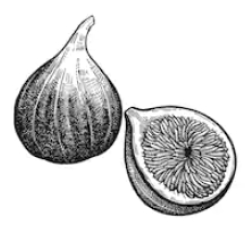
\includegraphics[width=2.5in]{fig1}
%\caption{Simulation results for the network.}
%\label{fig_1}
%\end{figure}

%Fig. 2(a) and 2(b) is an example of a double column floating figure using two subfigures.
% (The subfig.sty package must be loaded for this to work.)
% The subfigure $\backslash${\tt{label}} commands are set within each subfloat command,
% and the $\backslash${\tt{label}} for the overall figure must come after $\backslash${\tt{caption}}.
% $\backslash${\tt{hfil}} is used as a separator to get equal spacing.
% The combined width of all the parts of the figure should do not exceed the text width or a line break will occur.
%
%\begin{figure*}[!t]
%\centering
%\subfloat[]{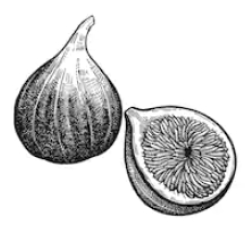
\includegraphics[width=2.5in]{fig1}%
%\label{fig_first_case}}
%\hfil
%\subfloat[]{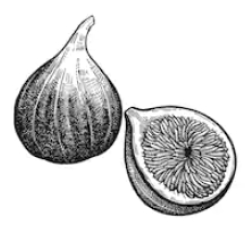
\includegraphics[width=2.5in]{fig1}%
%\label{fig_second_case}}
%\caption{Dae. Ad quatur autat ut porepel itemoles dolor autem fuga. Bus quia con nessunti as remo di quatus non perum que nimus. (a) Case I. (b) Case II.}
%\label{fig_sim}
%\end{figure*}

%Note that often IEEE papers with multi-part figures do not place the labels within the image itself (using the optional argument to $\backslash${\tt{subfloat}}[]), but instead will
% reference/describe all of them (a), (b), etc., within the main caption.
% Be aware that for subfig.sty to generate the (a), (b), etc., subfigure
% labels, the optional argument to $\backslash${\tt{subfloat}} must be present. If a
% subcaption is not desired, leave its contents blank,
% e.g.,$\backslash${\tt{subfloat}}[].


 

%\section{Tables}
%Note that, for IEEE-style tables, the
% $\backslash${\tt{caption}} command should come BEFORE the table. Table captions use title case. Articles (a, an, the), coordinating conjunctions (and, but, for, or, nor), and most short prepositions are lowercase unless they are the first or last word. Table text will default to $\backslash${\tt{footnotesize}} as
% the IEEE normally uses this smaller font for tables.
% The $\backslash${\tt{label}} must come after $\backslash${\tt{caption}} as always.
 
%\begin{table}[!t]
%\caption{An Example of a Table\label{tab:table1}}
%\centering
%\begin{tabular}{|c||c|}
%\hline
%One & Two\\
%\hline
%Three & Four\\
%\hline
%\end{tabular}
%\end{table}

%\section{Algorithms}
%Algorithms should be numbered and include a short title. They are set off from the text with rules above and below the title and after the last line.

%\begin{algorithm}[H]
%\caption{Weighted Tanimoto ELM.}\label{alg:alg1}
%\begin{algorithmic}
%\STATE 
%\STATE {\textsc{TRAIN}}$(\mathbf{X} \mathbf{T})$
%\STATE \hspace{0.5cm}$ \textbf{select randomly } W \subset \mathbf{X}  $
%\STATE \hspace{0.5cm}$ N_\mathbf{t} \gets | \{ i : \mathbf{t}_i = \mathbf{t} \} | $ \textbf{ for } $ \mathbf{t}= -1,+1 $
%\STATE \hspace{0.5cm}$ B_i \gets \sqrt{ \textsc{max}(N_{-1},N_{+1}) / N_{\mathbf{t}_i} } $ \textbf{ for } $ i = 1,...,N $
%\STATE \hspace{0.5cm}$ \hat{\mathbf{H}} \gets  B \cdot (\mathbf{X}^T\textbf{W})/( \mathbb{1}\mathbf{X} + \mathbb{1}\textbf{W} - \mathbf{X}^T\textbf{W} ) $
%\STATE \hspace{0.5cm}$ \beta \gets \left ( I/C + \hat{\mathbf{H}}^T\hat{\mathbf{H}} \right )^{-1}(\hat{\mathbf{H}}^T B\cdot \mathbf{T})  $
%\STATE \hspace{0.5cm}\textbf{return}  $\textbf{W},  \beta $
%\STATE 
%\STATE {\textsc{PREDICT}}$(\mathbf{X} )$
%\STATE \hspace{0.5cm}$ \mathbf{H} \gets  (\mathbf{X}^T\textbf{W} )/( \mathbb{1}\mathbf{X}  + \mathbb{1}\textbf{W}- \mathbf{X}^T\textbf{W}  ) $
%\STATE \hspace{0.5cm}\textbf{return}  $\textsc{sign}( \mathbf{H} \beta )$
%\end{algorithmic}
%\label{alg1}
%\end{algorithm}

%Que sunt eum lam eos si dic to estist, culluptium quid qui nestrum nobis reiumquiatur minimus minctem. Ro moluptat fuga. Itatquiam ut laborpo rersped exceres vollandi repudaerem. Ulparci sunt, qui doluptaquis sumquia ndestiu sapient iorepella sunti veribus. Ro moluptat fuga. Itatquiam ut laborpo rersped exceres vollandi repudaerem. 
%\section{Mathematical Typography \\ and Why It Matters}

%Typographical conventions for mathematical formulas have been developed to {\bf provide uniformity and clarity of presentation across mathematical texts}. This enables the readers of those texts to both understand the author's ideas and to grasp new concepts quickly. While software such as \LaTeX \ and MathType\textsuperscript{\textregistered} can produce aesthetically pleasing math when used properly, it is also very easy to misuse the software, potentially resulting in incorrect math display.

%IEEE aims to provide authors with the proper guidance on mathematical typesetting style and assist them in writing the best possible article. As such, IEEE has assembled a set of examples of good and bad mathematical typesetting \cite{ref1,ref2,ref3,ref4,ref5}. 

%Further examples can be found at \url{http://journals.ieeeauthorcenter.ieee.org/wp-content/uploads/sites/7/IEEE-Math-Typesetting-Guide-for-LaTeX-Users.pdf}

%\subsection{Display Equations}
%The simple display equation example shown below uses the ``equation'' environment. To number the equations, use the $\backslash${\tt{label}} macro to create an identifier for the equation. LaTeX will automatically number the equation for you.
%\begin{equation}
%\label{deqn_ex1}
%x = \sum_{i=0}^{n} 2{i} Q.
%\end{equation}

%\noindent is coded as follows:
%\begin{verbatim}
%\begin{equation}
%\label{deqn_ex1}
%x = \sum_{i=0}^{n} 2{i} Q.
%\end{equation}
%\end{verbatim}

%To reference this equation in the text use the $\backslash${\tt{ref}} macro. 
%Please see (\ref{deqn_ex1})\\
%\noindent is coded as follows:
%\begin{verbatim}
%Please see (\ref{deqn_ex1})\end{verbatim}

%\subsection{Equation Numbering}
%{\bf{Consecutive Numbering:}} Equations within an article are numbered consecutively from the beginning of the
%article to the end, i.e., (1), (2), (3), (4), (5), etc. Do not use roman numerals or section numbers for equation numbering.

%\noindent {\bf{Appendix Equations:}} The continuation of consecutively numbered equations is best in the Appendix, but numbering
% as (A1), (A2), etc., is permissible.\\

%\noindent {\bf{Hyphens and Periods}}: Hyphens and periods should not be used in equation numbers, i.e., use (1a) rather than
%(1-a) and (2a) rather than (2.a) for subequations. This should be consistent throughout the article.

%\subsection{Multi-Line Equations and Alignment}
%Here we show several examples of multi-line equations and proper alignments.

%\noindent {\bf{A single equation that must break over multiple lines due to length with no specific alignment.}}
%\begin{multline}
%\text{The first line of this example}\\
%\text{The second line of this example}\\
%\text{The third line of this example}
%\end{multline}

%\noindent is coded as:
%\begin{verbatim}
%\begin{multline}
%\text{The first line of this example}\\
%\text{The second line of this example}\\
%\text{The third line of this example}
%\end{multline}
%\end{verbatim}

%\noindent {\bf{A single equation with multiple lines aligned at the = signs}}
%\begin{align}
%a &= c+d \\
%b &= e+f
%\end{align}
%\noindent is coded as:
%\begin{verbatim}
%\begin{align}
%a &= c+d \\
%b &= e+f
%\end{align}
%\end{verbatim}

%The {\tt{align}} environment can align on multiple  points as shown in the following example:
%\begin{align}
%x &= y & X & =Y & a &=bc\\
%x' &= y' & X' &=Y' &a' &=bz
%\end{align}
%\noindent is coded as:
%\begin{verbatim}
%\begin{align}
%x &= y & X & =Y & a &=bc\\
%x' &= y' & X' &=Y' &a' &=bz
%\end{align}
%\end{verbatim}





%\subsection{Subnumbering}
%The amsmath package provides a {\tt{subequations}} environment to facilitate subnumbering. An example:

%\begin{subequations}\label{eq:2}
%\begin{align}
%f&=g \label{eq:2A}\\
%f' &=g' \label{eq:2B}\\
%\mathcal{L}f &= \mathcal{L}g \label{eq:2c}
%\end{align}
%\end{subequations}

%\noindent is coded as:
%\begin{verbatim}
%\begin{subequations}\label{eq:2}
%\begin{align}
%f&=g \label{eq:2A}\\
%f' &=g' \label{eq:2B}\\
%\mathcal{L}f &= \mathcal{L}g \label{eq:2c}
%\end{align}
%\end{subequations}

%\end{verbatim}

%\subsection{Matrices}
%There are several useful matrix environments that can save you some keystrokes. See the example coding below and the output.

%\noindent {\bf{A simple matrix:}}
%\begin{equation}
%\begin{matrix}  0 &  1 \\ 
%1 &  0 \end{matrix}
%\end{equation}
%is coded as:
%\begin{verbatim}
%\begin{equation}
%\begin{matrix}  0 &  1 \\ 
%1 &  0 \end{matrix}
%\end{equation}
%\end{verbatim}

%\noindent {\bf{A matrix with parenthesis}}
%\begin{equation}
%\begin{pmatrix} 0 & -i \\
% i &  0 \end{pmatrix}
%\end{equation}
%is coded as:
%\begin{verbatim}
%\begin{equation}
%\begin{pmatrix} 0 & -i \\
% i &  0 \end{pmatrix}
%\end{equation}
%\end{verbatim}

%\noindent {\bf{A matrix with square brackets}}
%\begin{equation}
%\begin{bmatrix} 0 & -1 \\ 
%1 &  0 \end{bmatrix}
%\end{equation}
%is coded as:
%\begin{verbatim}
%\begin{equation}
%\begin{bmatrix} 0 & -1 \\ 
%1 &  0 \end{bmatrix}
%\end{equation}
%\end{verbatim}

%\noindent {\bf{A matrix with curly braces}}
%\begin{equation}
%\begin{Bmatrix} 1 &  0 \\ 
%0 & -1 \end{Bmatrix}
%\end{equation}
%is coded as:
%\begin{verbatim}
%\begin{equation}
%\begin{Bmatrix} 1 &  0 \\ 
%0 & -1 \end{Bmatrix}
%\end{equation}\end{verbatim}

%\noindent {\bf{A matrix with single verticals}}
%\begin{equation}
%\begin{vmatrix} a &  b \\ 
%c &  d \end{vmatrix}
%\end{equation}
%is coded as:
%\begin{verbatim}
%\begin{equation}
%\begin{vmatrix} a &  b \\ 
%c &  d \end{vmatrix}
%\end{equation}\end{verbatim}

%\noindent {\bf{A matrix with double verticals}}
%\begin{equation}
%\begin{Vmatrix} i &  0 \\ 
%0 & -i \end{Vmatrix}
%\end{equation}
%is coded as:
%\begin{verbatim}
%\begin{equation}
%\begin{Vmatrix} i &  0 \\ 
%0 & -i \end{Vmatrix}
%\end{equation}\end{verbatim}

%\subsection{Arrays}
%The {\tt{array}} environment allows you some options for matrix-like equations. You will have to manually key the fences, but there are other options for alignment of the columns and for setting horizontal and vertical rules. The argument to {\tt{array}} controls alignment and placement of vertical rules.

%A simple array
%\begin{equation}
%\left(
%\begin{array}{cccc}
%a+b+c & uv & x-y & 27\\
%a+b & u+v & z & 134
%\end{array}\right)
%\end{equation}
%is coded as:
%\begin{verbatim}
%\begin{equation}
%\left(
%\begin{array}{cccc}
%a+b+c & uv & x-y & 27\\
%a+b & u+v & z & 134
%\end{array} \right)
%\end{equation}
%\end{verbatim}

%A slight variation on this to better align the numbers in the last column
%\begin{equation}
%\left(
%\begin{array}{cccr}
%a+b+c & uv & x-y & 27\\
%a+b & u+v & z & 134
%\end{array}\right)
%\end{equation}
%is coded as:
%\begin{verbatim}
%\begin{equation}
%\left(
%\begin{array}{cccr}
%a+b+c & uv & x-y & 27\\
%a+b & u+v & z & 134
%\end{array} \right)
%\end{equation}
%\end{verbatim}

%An array with vertical and horizontal rules
%\begin{equation}
%\left( \begin{array}{c|c|c|r}
%a+b+c & uv & x-y & 27\\ \hline
%a+b & u+v & z & 134
%\end{array}\right)
%\end{equation}
%is coded as:
%\begin{verbatim}
%\begin{equation}
%\left(
%\begin{array}{c|c|c|r}
%a+b+c & uv & x-y & 27\\
%a+b & u+v & z & 134
%\end{array} \right)
%\end{equation}
%\end{verbatim}
%Note the argument now has the pipe "$\vert$" included to indicate the placement of the vertical rules.


%\subsection{Cases Structures}
%Many times cases can be miscoded using the wrong environment, i.e., {\tt{array}}. Using the {\tt{cases}} environment will save keystrokes (from not having to type the $\backslash${\tt{left}}$\backslash${\tt{lbrace}}) and automatically provide the correct column alignment.
%\begin{equation*}
%{z_m(t)} = \begin{cases}
%1,&{\text{if}}\ {\beta }_m(t) \\ 
%{0,}&{\text{otherwise.}} 
%\end{cases}
%\end{equation*}
%\noindent is coded as follows:
%\begin{verbatim}
%\begin{equation*}
%{z_m(t)} = 
%\begin{cases}
%1,&{\text{if}}\ {\beta }_m(t),\\ 
%{0,}&{\text{otherwise.}} 
%\end{cases}
%\end{equation*}
%\end{verbatim}
%\noindent Note that the ``\&'' is used to mark the tabular alignment. This is important to get  proper column alignment. Do not use $\backslash${\tt{quad}} or other fixed spaces to try and align the columns. Also, note the use of the $\backslash${\tt{text}} macro for text elements such as ``if'' and ``otherwise.''

%\subsection{Function Formatting in Equations}
%Often, there is an easy way to properly format most common functions. Use of the $\backslash$ in front of the function name will in most cases, provide the correct formatting. When this does not work, the following example provides a solution using the $\backslash${\tt{text}} macro:

%\begin{equation*} 
%  d_{R}^{KM} = \underset {d_{l}^{KM}} {\text{arg min}} \{ d_{1}^{KM},\ldots,d_{6}^{KM}\}.
%\end{equation*}

%\noindent is coded as follows:
%\begin{verbatim}
%\begin{equation*} 
% d_{R}^{KM} = \underset {d_{l}^{KM}} 
% {\text{arg min}} \{ d_{1}^{KM},
% \ldots,d_{6}^{KM}\}.
%\end{equation*}
%\end{verbatim}

%\subsection{ Text Acronyms Inside Equations}
%This example shows where the acronym ``MSE" is coded using $\backslash${\tt{text\{\}}} to match how it appears in the text.

%\begin{equation*}
% \text{MSE} = \frac {1}{n}\sum _{i=1}^{n}(Y_{i} - \hat {Y_{i}})^{2}
%\end{equation*}

%\begin{verbatim}
%\begin{equation*}
% \text{MSE} = \frac {1}{n}\sum _{i=1}^{n}
%(Y_{i} - \hat {Y_{i}})^{2}
%\end{equation*}
%\end{verbatim}

%\section{Conclusion}
%The conclusion goes here.


%\section*{Acknowledgments}
%This should be a simple paragraph before the References to thank those individuals and institutions who have supported your work on this article.



%{\appendix[Proof of the Zonklar Equations]
%Use $\backslash${\tt{appendix}} if you have a single appendix:
%Do not use $\backslash${\tt{section}} anymore after $\backslash${\tt{appendix}}, only $\backslash${\tt{section*}}.
%If you have multiple appendixes use $\backslash${\tt{appendices}} then use $\backslash${\tt{section}} to start each appendix.
%You must declare a $\backslash${\tt{section}} before using any $\backslash${\tt{subsection}} or using $\backslash${\tt{label}} ($\backslash${\tt{appendices}} by itself
% starts a section numbered zero.)}



%{\appendices
%\section*{Proof of the First Zonklar Equation}
%Appendix one text goes here.
% You can choose not to have a title for an appendix if you want by leaving the argument blank
%\section*{Proof of the Second Zonklar Equation}
%Appendix two text goes here.}




%\section{References Section}
%You can use a bibliography generated by BibTeX as a .bbl file.
% BibTeX documentation can be easily obtained at:
% http://mirror.ctan.org/biblio/bibtex/contrib/doc/
% The IEEEtran BibTeX style support page is:
% http://www.michaelshell.org/tex/ieeetran/bibtex/
 
 % argument is your BibTeX string definitions and bibliography database(s)
%\bibliography{IEEEabrv,../bib/paper}
%
%\section{Simple References}
%You can manually copy in the resultant .bbl file and set second argument of $\backslash${\tt{begin}} to the number of references
% (used to reserve space for the reference number labels box).

%\begin{thebibliography}{1}
%\bibliographystyle{IEEEtran}

%\bibitem{ref1}
%{\it{Mathematics Into Type}}. American Mathematical Society. [Online]. Available: https://www.ams.org/arc/styleguide/mit-2.pdf

%\bibitem{ref2}
%T. W. Chaundy, P. R. Barrett and C. Batey, {\it{The Printing of Mathematics}}. London, U.K., Oxford Univ. Press, 1954.

%\bibitem{ref3}
%F. Mittelbach and M. Goossens, {\it{The \LaTeX Companion}}, 2nd ed. Boston, MA, USA: Pearson, 2004.

%\bibitem{ref4}
%G. Gr\"atzer, {\it{More Math Into LaTeX}}, New York, NY, USA: Springer, 2007.

%\bibitem{ref5}M. Letourneau and J. W. Sharp, {\it{AMS-StyleGuide-online.pdf,}} American Mathematical Society, Providence, RI, USA, [Online]. Available: http://www.ams.org/arc/styleguide/index.html

%\bibitem{ref6}
%H. Sira-Ramirez, ``On the sliding mode control of nonlinear systems,'' \textit{Syst. Control Lett.}, vol. 19, pp. 303--312, 1992.

%\bibitem{ref7}
%A. Levant, ``Exact differentiation of signals with unbounded higher derivatives,''  in \textit{Proc. 45th IEEE Conf. Decis.
%Control}, San Diego, CA, USA, 2006, pp. 5585--5590. DOI: 10.1109/CDC.2006.377165.

%\bibitem{ref8}
%M. Fliess, C. Join, and H. Sira-Ramirez, ``Non-linear estimation is easy,'' \textit{Int. J. Model., Ident. Control}, vol. 4, no. 1, pp. 12--27, 2008.

%\bibitem{ref9}
%R. Ortega, A. Astolfi, G. Bastin, and H. Rodriguez, ``Stabilization of food-chain systems using a port-controlled Hamiltonian description,'' in \textit{Proc. Amer. Control Conf.}, Chicago, IL, USA,
%2000, pp. 2245--2249.

%\end{thebibliography}


%\newpage

%\section{Biography Section}
%If you have an EPS/PDF photo (graphicx package needed), extra braces are
% needed around the contents of the optional argument to biography to prevent
% the LaTeX parser from getting confused when it sees the complicated
% $\backslash${\tt{includegraphics}} command within an optional argument. (You can create
% your own custom macro containing the $\backslash${\tt{includegraphics}} command to make things
% simpler here.)
 
%\vspace{11pt}

%\bf{If you include a photo:}\vspace{-33pt}
%\begin{IEEEbiography}[{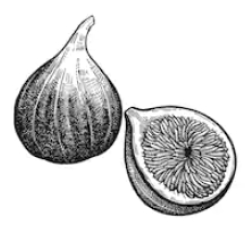
\includegraphics[width=1in,height=1.25in,clip,keepaspectratio]{fig1}}]{Michael Shell}
%Use $\backslash${\tt{begin\{IEEEbiography\}}} and then for the 1st argument use $\backslash${\tt{includegraphics}} to declare and link the author photo.
%Use the author name as the 3rd argument followed by the biography text.
%\end{IEEEbiography}

%\vspace{11pt}

%\bf{If you will not include a photo:}\vspace{-33pt}
%\begin{IEEEbiographynophoto}{John Doe}
%Use $\backslash${\tt{begin\{IEEEbiographynophoto\}}} and the author name as the argument followed by the biography text.
%\end{IEEEbiographynophoto}


~~

\newpage

{\small\bibliographystyle{IEEEtran}  %
%\bibliography{../../books/phd-thesis/backmatter/references}}
\bibliography{rb5-paper}}  


\vfill

\end{document}


